% ===== 原文 pp.85--89 =====
% [原文 p.85]
% （承接 tr06b 末尾：「……这是看清余维 4 算子」）
应当依赖于 $\fg$ 的这种表示。进一步约化到 4d 给出一个半 BPS 的 Wilson 圈，它测量相应规范场 $A_\gamma$ 沿 $L$ 的和乐（holonomy），再加上来自标量超伙伴（scalar superpartners）的某些贡献以确保超对称性：
\begin{equation}
    W_{\gamma,R}=\Tr_R\left(\mathrm{Pexp}\int_L\left(A_\gamma+\mathrm{scalars}_\gamma\right)\right).
    \tag{8.3}
\end{equation}
规范群 $G_\gamma$ 与 Wilson 圈只依赖于 $\gamma$ 的同伦类（homotopy class）。
% [Tutor Note: p.85 (8.3) 里 $\mathrm{Pexp}$ 是路径排序指数（path-ordered exponential），$\mathrm{scalars}_\gamma$ 指与 $A_\gamma$ 同属一个 $\cN=2$ 矢量多重态、沿 $L$ 匹配的标量组合；把它们算进去正是为了保持半 BPS 性------只取规范场会破坏超对称。核对：$\Tr_R$ 取表示 $R$ 的迹，因此 $W_{\gamma,R}$ 在 $G_\gamma$ 下不变；弱耦合时它 $\to\Tr_R(\id)=$ 表示的维数（$R$ 取基本表示时 $=N$），这是判读弱耦合极限的一个可用锚点。]

在 2d CFT 一侧，相应的对象是沿 $\gamma$ 的某个 1d 拓扑缺陷，称为退化 Verlinde 圈算子（degenerate Verlinde loop operator）。Verlinde 圈被构造为顶点算子 $V_\omega$ 的单值（monodromy）。对应于 $W_{\gamma,R}$ 的具体选择是取动量 $\omega=-b^{\pm1}\Omega_R$，其中 $\pm$ 号取决于所选的圆周 $L$，而 $\Omega_R$ 是表示 $R$ 的最高权。\footnote{权位于 $\fh^*$ 中；借助 Killing 形式，我们把它与 Cartan 子代数 $\fh\subset\fg$ 等同起来。} 对这个 $\omega$ 的选择，顶点算子 $V_\omega$ 是退化的，意思是它被 W 代数生成元的各种组合湮灭。顺便说，最一般的退化动量 $\omega=-b\Omega-b^{-1}\Omega'$ 对应于沿两个允许的圆周同时插入 Wilson 圈。

对应对的具体检验是直截了当的。Wilson 圈与超对称局域化 [10] 相容，并在 (1.7) 中插入一个简单的、与 $a$ 有关的因子。Verlinde 圈 $\cL_\gamma$ 作用在沿 $\gamma$ 插入的一组完备态上是对角的，因而在关联函数 (1.9) 中只作为内动量 $\alpha$（与 $a$ 有关）的函数出现。二者相吻合：
\begin{equation}
\begin{aligned}
    \langle W_{\gamma,R}\rangle^{\mathsf{T}(\fg,C,D)}_{S^4_b}
    &=\int\dd a\;\Tr_R(e^{a_\gamma})\,Z_{\mathrm{cl}}(a,q,\bar q)\,Z_{\text{one-loop}}(a)Z_{\mathrm{inst}}(a,q)Z_{\mathrm{inst}}(a,\bar q)\\
    &=\int\dd\alpha\;f(\alpha)\,C(\alpha)\cF(\alpha,q)\cF(\alpha,\bar q)\\
    &=\left\langle\hat V_{\mu_1}\ldots\hat V_{\mu_n}\cL_\gamma\right\rangle^{\mathrm{Toda}(\fg)}_{\C}.
\end{aligned}
    \tag{8.4}
\end{equation}
% [Tutor Note: p.85 (8.4) 的三行是同一个量的三种表述：第一行是 $S^4_b$ 上的局域化积分（经典作用 + 单圈行列式 + 两半的瞬子贡献），第二行把它归并为测度 $f(\alpha)$、三点函数 $C(\alpha)$ 与两半的共形块 $\cF$ 之积，第三行是 Toda 关联函数。核对要点：第一行只有一处 $\Tr_R(e^{a_\gamma})$，它对应第三行的 $\cL_\gamma$；$Z_{\mathrm{cl}}$ 给出与 $q,\bar q$ 相关的因子，而在第二行中 $q$ 只出现在 $\cF$ 中。]

\para{双子圈算子。} 现在考虑 $C$ 的一个裤子分解，它不把 $\gamma$ 包含在其切割之中。2d CFT 一侧仍由沿 $\gamma$ 的 Verlinde 圈给出，但它在给定的共形块基下的表达式不再是对角的：它等于
\begin{equation}
    \left\langle\hat V_{\mu_1}\ldots\hat V_{\mu_n}\cL_\gamma\right\rangle^{\mathrm{Toda}(\fg)}_{\C}
    =\int\dd\alpha\;C(\alpha)\cF(\alpha,q)\sum_h\cL_\gamma(\alpha,\alpha+h)\cF(\alpha+h,\bar q)
    \tag{8.5}
\end{equation}
其中 $h$ 取遍与 $R$ 的权有关的一个有限集合，\footnote{退化算子 $V_\omega$ 与另一个顶点算子的融合只有有限多项。} 4d 中相应的圈算子在这个 S 对偶框架下被描述为 't Hooft 圈或双子圈，而不是 Wilson 圈。't Hooft 圈不像 Wilson 圈 (8.3) 那样由路径积分中的一个插入来定义，而是通过给规范场强加一个奇异的边界条件来定义，该条件规定围绕 $L$ 的二维球面 $S^2$ 上具有非零的单极荷 $\frac{1}{2\pi}\int F$。双子圈还额外地包含沿同一圆周 $L$ 的一个 Wilson 圈插入。路径积分的范围包括这类奇异

% [原文 p.86]
场构型，而不再是通常的构型；超对称局域化仍然适用 [501]，并重现 (8.5)，只要正确地计入单极气泡（monopole bubbling）[503--508]。

有趣的是，Verlinde 圈必须推广为 Verlinde 网络（涉及退化顶点算子的融合），才能重现具有最一般电磁荷的半 BPS 双子圈 [46,51,52,516]。

\para{线算子的代数。} 鉴于 (8.5)，双子圈或 Verlinde 网络可以理解为作用在内动量 $\alpha$ 的函数上的差分算子，或等价地作用在 Coulomb 分支 $\cB$ 上的函数。在不同的纬度（latitude）$y^5$ 处插入双子圈给出差分算子的乘积，这个乘积是非对易的，因为这些圈无法在保持超对称的同时重排。圈算子的 OPE 给出 skein 关系（skein relations），把这些乘积表示成双子圈的线性组合，并定义一个圈算子代数 $\mathfrak{A}_{\epsilon_1,\epsilon_2}$（回忆 $\epsilon_1=b/r$、$\epsilon_2=1/(rb)$）。Teschner [309,517] 很早就强调了这一代数在 AGT 对应中的重要性；综述见 [489,518]。更早的工作 [519] 集中于 4d $\cN=4$ SYM。
% [Tutor Note: p.86 的 $\epsilon_1=b/r$、$\epsilon_2=1/(rb)$ 可用来核对 NS 极限：$\epsilon_1\epsilon_2=1/r^2$、$\epsilon_1/\epsilon_2=b^2$，故 $r=1/\sqrt{\epsilon_1\epsilon_2}$、$b=\sqrt{\epsilon_1/\epsilon_2}$。于是"$\epsilon_1,\epsilon_2\to0$ 即 $r\to\infty$"（$S^4_b$ 半径发散、回到平坦空间）与"$\epsilon_2\to0$ 而 $\epsilon_1$ 固定"（NS 极限）分别对应 $b$ 按 $\sqrt{\epsilon_1/\epsilon_2}$ 发散。这也解释了为什么 NS 极限下 $S^4_b$ 退化为 $\R^2\times S^2_b$：$r\to\infty$ 只放大两个方向。]

$C$ 的每个裤子分解都给出 $\mathfrak{A}_{\epsilon_1,\epsilon_2}$ 的一个差分算子表示，其中某些圈被对角化 (8.4)，而另一些仍是非对角的 (8.5)。把不同裤子分解下的共形块联系起来的模核（modular kernels），正是在各种圈算子的本征基之间做映射，它们可以从 $\mathfrak{A}_{\epsilon_1,\epsilon_2}$ 算出来。本征基本身（即瞬子配分函数）则是一个可求解的 Riemann--Hilbert 型问题的解。它们 $\epsilon_1,\epsilon_2\to0$ 的极限就是低能预势 (5.30)。$\mathfrak{A}_{\epsilon_1,\epsilon_2}$ 中隐藏的这一切丰富内容，使 [309] 的作者把它称为 $\mathsf{T}(\fg,C,D)$ 的"非微扰骨架"（non-perturbative skeleton）。

在代数 $\mathfrak{A}_{\epsilon_1,\epsilon_2}$ 的 Nekrasov--Shatashvili（NS）极限 $\epsilon_2\to0$ 下，差分算子变成 $\cB$ 上的微分算子，而在经典极限 $\epsilon_1,\epsilon_2\to0$ 下它们进一步变成 $\cB$ 上的环面纤维化（torus fibration）的坐标。\footnote{类似于量子力学中的动量 $p\sim\ii\partial_x$ 在经典力学中是一个坐标。} 几何在 NS 极限下变简单：$S^4_b$ 退化为 $\R^2\times S^2_b$。在沿 $S^2_b$ 赤道的圈附近，几何是 $\R^3\times_b S^1$，其中绕 $S^1$ 的周期性被扭过，而在经典极限下这个扭被去掉。正是这个几何在 [167,502,510,520--523] 中被考虑过（关于"framed BPS 态"）。在未扭的 $\R^3\times S^1$ 上，圈算子的真空期望值定义了 $\R^3\times S^1$ 上 class S 理论的 Coulomb 分支 $\cM$ 上的坐标，而 $\cM$ 就是前述 $\cB$ 上的环面纤维化。$\R^3\times_b S^1$ 的扭曲周期性把这个坐标代数量子化成微分算子代数，即 $\mathfrak{A}_{\epsilon_1,\epsilon_2}$ 的 NS 极限。

如 (3.14) 附近所述，$\R^3\times S^1$ 上的 Coulomb 分支 $\cM$ 可以等价地看作 $C$ 上的 Hitchin 模空间，或者看作 $C$ 上平坦 $G_\C$ 联络的模空间（其中 $G_\C$ 的李代数是 $\fg$ 的复化）。最后这个观点与 9.3 小节讨论的 3d/3d 对应很契合，后者涉及 $G_\C$ Chern--Simons 理论。关于 Hitchin 系统、opers 与 $\cM$ 上 Darboux 坐标的进一步工作包括 [50,343,356,366,415,488,524--535]（其中一些在 [536] 中有综述）；另一种

% [原文 p.87]
技术基于谱网络（spectral networks），把 $C$ 上的平坦联络阿贝尔化 [537--549]；另见 [49,550--552]。

\subsection{面算子}

面算子在 [458] 中有综述（早期文献见 [553,554]）。与 $S^4_b$ 上的超对称局域化相容的面算子，可以沿两个在极点相交的压扁球面（squashed spheres）插入，或沿某些二维环面插入，后者用 $\R^5$ 的笛卡尔坐标写出如下：
\begin{equation}
\begin{aligned}
    S^4_b&:=\left\{y_5^2+b^2(y_1^2+y_2^2)+b^{-2}(y_3^2+y_4^2)=r^2\right\},\\
    S^2_b&:=\left\{y_1=y_2=0,\;y_5^2+b^{-2}(y_3^2+y_4^2)=r^2\right\},\\
    S^2_{1/b}&:=\left\{y_5^2+b^2(y_1^2+y_2^2)=r^2,\;y_3=y_4=0\right\},\\
    T^2_{\theta,\varphi}&:=\left\{y_5=r\cos\theta,\;y_1^2+y_2^2=(rb^{-1}\sin\theta\cos\varphi)^2,\;y_3^2+y_4^2=(rb\sin\theta\sin\varphi)^2\right\}.
\end{aligned}
    \tag{8.6}
\end{equation}
% [Tutor Note: p.87 (8.6) 的最后一行可当场验算：把 $T^2_{\theta,\varphi}$ 的三个式子代入 $S^4_b$ 的定义得 $y_5^2+b^2(y_1^2+y_2^2)+b^{-2}(y_3^2+y_4^2)=r^2\cos^2\theta+r^2\sin^2\theta\cos^2\varphi+r^2\sin^2\theta\sin^2\varphi=r^2$，故该二维环面确实落在 $S^4_b$ 上。同样可核 $S^2_b,S^2_{1/b}$ 分别是 $S^4_b$ 与 $y_1=y_2=0$、$y_3=y_4=0$ 的交（即两个"压扁球面"，半径都为 $r$）；原文"两个在极点相交的压扁球面"即指 $S^2_b$ 与 $S^2_{1/b}$ 在 $y_5=\pm r$ 处相遇。]

后一种情形尚未被研究过，因此我们这里只集中于球面；在球面上，面算子保持 4d $\cN=2$ 的一个 2d $\cN=(2,2)$ 子代数。这类算子或者来自 $C$ 中一点 $z$ 处的 $\cX(\fg)$ 余维 4 算子，或者来自包裹整个 $C$ 的余维 2 算子。（另见 [516] 关于面算子组成的泡沫（foams）、[555,556] 关于对偶缺陷、[557] 关于全息进路。）第一类面算子的耦合空间正好就是 UV 曲线 $C$，因此它直接从 4d $\cN=2$ 理论给出 $C$ 的一个定义。

\para{涡旋弦算子。} 我们从这样的面算子开始：它来自 6d 理论的余维 4 算子，该算子放在一点 $z\in C$ 处，并落在两个可能的球面 $S^2_b$（下文记号为"$+$"）或 $S^2_{1/b}$（下文记号为"$-$"）之一上。这类算子有时称为 M2 膜面算子（M2-brane surface operators），因为它在 class S 理论的 M 理论构造中来自额外 M2 膜的加入。若被 Higgs 的场具有非平凡的、依赖空间的剖面（profile），它们也可以通过 Higgsing 一个更大的 4d 理论而得到 [558--560]。它们在 AGT 中的解释在 [39,55--63,66--71,561,562] 中被探索，部分基于其精确配分函数，后者在 [69,503--576] 中研究过。同样的算子在对应的 5d 版本以及 $S^1\times S^3_b$ 版本中也很重要 [64,65,190,570,571,577--580]；关于这类面算子的其他考虑另见 [537,539,581--590]。

正如我们研究圈算子时学到的，余维 4 算子带有一个 $\fg$ 的表示 $R$ 的选择。在 2d CFT 一侧，我们因此想要一个由 $R$ 标记的点算子：自然的猜测是动量为 $\omega=-b^{\pm1}\Omega_R$ 的退化顶点算子 $V_\omega$，其中符号 $\pm$ 由我们在 4d 一侧使用哪个压扁二维球面决定。这提示一个等式
\begin{equation}
    \left\langle\text{surface operator}\right\rangle^{\mathsf{T}(\fg,C,D)}_{S^4_b}
    =\left\langle\hat V_{\mu_1}\ldots\hat V_{\mu_n}V_{-b^{\pm1}\Omega_R}\right\rangle^{\mathrm{Toda}(\fg)}_{\C}.
    \tag{8.7}
\end{equation}
右端可以写成由非退化顶点算子构成的 $(n+1)$ 点关联函数 $\langle\hat V_{\mu_1}\ldots\hat V_{\mu_{n+1}}\rangle$ 的解析延拓。该解析延拓

% [原文 p.88]
在相应的 class S 理论 $T'$ 中最早是在 [558] 里就 Lagrangian 情形得到理解的\footnote{对最一般的 class S 理论把这一情形澄清会是有益的。}：它相当于在 $T'$ 中考虑一个超对称的"涡旋弦"（vortex string）构型，其中某些超多重态标量获得集中在余维 2 上的、依赖空间的真空期望值。在低能极限下，非零标量把 $T'$ 的一些规范对称性 Higgs 到 $T$ 的那些，而该构型被一个位于理论 $T$ 中的面算子有效地描述。

\para{作为 4d--2d 耦合系统的描述。} 除了这种由 $\cX(\fg)$ 的余维 4 算子得到的涡旋弦构造之外，这些面算子还可以通过耦合一个生活在缺陷上的 2d $\cN=(2,2)$ 规范理论来描述。在此语境下，(8.7) 的左端就是压扁球面上 4d--2d 耦合系统的配分函数。一个简单的例子是 $SU(2)$ $N_f=4$ SQCD、且缺陷由第 $K$ 个对称表示（symmetric representation）标记的情形。此时该 2d 理论由手征多重态组成：它们构成 4d 味群与规范群的双重态表示（doublet representations），以及 2d $U(K)$ 规范群的基本与反基本表示：
\begin{equation}
    Z_{S^2_b\subset S^4_b}\left[\,
    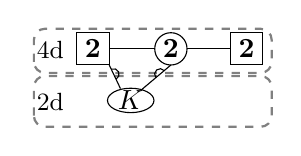
\begin{tikzpicture}[scale=1.0,baseline=(current bounding box.center)]
      % 两个虚线圆角框（上 4d、下 2d）
      \draw[gray,dashed,thick,rounded corners=4pt] (0,0.70) rectangle (3.02,1.26);
      \draw[gray,dashed,thick,rounded corners=4pt] (0,0.015) rectangle (3.02,0.66);
      % 区标签
      \node[font=\small] at (0.21,0.99) {4d};
      \node[font=\small] at (0.21,0.33) {2d};
      % 4d 箭图：方框 2 -- 圆 2 -- 方框 2
      \draw (0.545,0.805) rectangle (0.955,1.215);
      \node at (0.75,1.005) {\textbf{2}};
      \draw (1.74,1.005) circle (0.205);
      \node at (1.74,1.005) {\textbf{2}};
      \draw (2.495,0.805) rectangle (2.905,1.215);
      \node at (2.70,1.005) {\textbf{2}};
      \draw (0.955,1.005) -- (1.535,1.005);
      \draw (1.945,1.005) -- (2.495,1.005);
      % 2d 的 U(K) 结点
      \draw (1.23,0.35) ellipse (0.295 and 0.155);
      \node at (1.23,0.35) {$K$};
      % 两条穿过界面的斜线
      \draw (0.955,0.805) -- (1.10,0.50);
      \draw (1.74,0.80) -- (1.36,0.48);
      % 界面处的小弧（跨在斜线上）
      \draw (1.013,0.683) ++(-64.6:0.07) arc[start angle=-64.6, end angle=115.4, radius=0.07];
      \draw (1.603,0.683) ++(39.8:0.07) arc[start angle=39.8, end angle=219.8, radius=0.07];
    \end{tikzpicture}
    \,\right]
    =\left\langle\hat V_{\mu_1}\hat V_{\mu_2}\hat V_{\mu_3}\hat V_{\mu_4}V_{-Kb/2}\right\rangle^{\text{Liouville}}_{S^2}.
    \tag{8.8}
\end{equation}
% [Tutor Note: p.88 (8.8) 是编号公式而内容是示意图（拓扑弦的 tinkertoy 记号），故按 STYLE_GUIDE §6bis 用 TikZ 重画。读图约定：方框 = 带两个基本超多重态的 $SU(2)$ 味群，圆圈 = 被规范的 $SU(2)$，椭圆 $K$ = 2d 规范群 $U(K)$；上虚框标 4d、下虚框标 2d，界面上的两条斜线与小弧表示 2d 缺陷与 4d 箭图两处结点的耦合。核对左右两端：4d 一侧有 4 个方框端点（4 个穿刺点）$\leftrightarrow$ 右端 4 个 $\hat V_{\mu_i}$，2d 一侧的 $U(K)$ 给出第 5 个插入 $V_{-Kb/2}$，其动量与 $K$ 成线性关系，正对应 2d 规范群的 FI 参数。]

该式中的 $V_{-Kb/2}$ 的位置 $z$ 与 2d $U(K)$ 规范群的 Fayet--Iliopoulos（FI）参数相匹配。对 $\fsu(N)$ Lagrangian 理论中最一般的 $R$，这样的 2d 描述在 [68] 中被提出，并通过在规范理论中比较极限 $z\to z_i$ 与已知的 $V_{-b^{\pm1}\Omega_R}$ 和 $\hat V_{\mu_i}$ 的 OPE 而被检验。更一般的退化插入 $V_{-b\Omega-\Omega'/b}$ 翻译成交叉的缺陷（intersecting defects），并在缺陷相交的极点处带有额外的 0d 场 [69]。检验像 (8.8) 这样的等式时的一个重要困难，是计算来自 $S^4_b$ 极点的贡献 $Z_{\mathrm{inst,vort}}$，它同时涉及 4d 理论的瞬子与 2d 理论的涡旋 [574]。顺便说，在 $\epsilon_1,\epsilon_2\to0$ 的极限下，这个 Nekrasov 配分函数的 4d--2d 类比同时给出 4d 理论的有效预势 $F$ 与 2d 理论的有效扭曲超势 $\cW$，后者早先在 [55,565] 中得到：
\begin{equation}
    \log Z_{\mathrm{inst,vort}}=\frac{F}{\epsilon_1\epsilon_2}+\frac{\cW}{\epsilon_1}+O(1).
    \tag{8.9}
\end{equation}
% [Tutor Note: p.88 (8.9) 的量纲核对：4d 瞬子配分函数的 $\Omega$ 背景给出 $\log Z_{\mathrm{inst}}\sim F/(\epsilon_1\epsilon_2)$（$F$ 的量纲是 $1/\text{耦合}^2$），而 2d 涡旋部分给出 $\cW/\epsilon_1$------少一个 $\epsilon$ 因子正说明它来自 2d（缺陷上的）有效作用。取 $\epsilon_1,\epsilon_2\to0$ 时第二项比第一项次一阶，故保留到 $O(1)$ 就能同时读出 $F$ 与 $\cW$；这也是原文说"Nekrasov 配分函数的 4d--2d 类比"的原因。]

\para{Gukov--Witten 算子：单值缺陷与轨形。} 接下来我们讨论称为 M5 膜面算子的面算子，亦即余维 2 算子、或轨形面缺陷，它们在 [72--85,120,318,358,362,553,570,576,591--598] 中被研究，在 [359,360] 中则从小弦理论的观点研究。我们已经遇到过 $\cX(\fg)$ 的余维 2 缺陷，因为它们是施加在微分 $\phi_k$ 上某些边界条件的驯服穿刺点的来源。把这些余维 2 算子包裹在 $C$ 上，就给出对 4d 场施加某些奇异边界条件的面算子。具体地，这给出 Gukov--Witten（GW）面算子的 $\cN=2$ 版本 [553]，它们要求 4d 规范场 $A$ 在 $r\to0$ 时表现为 $A\sim\alpha\dd\theta$

% [原文 p.89]
其中 $\alpha\in\ft$ 是 $\fg$ 的 Cartan 代数中一个给定的元素，$(r,\theta)$ 是垂直于缺陷的极坐标。
% [Tutor Note: p.88--89 的 GW 面算子边界条件 $A\sim\alpha\dd\theta$ 即"单值缺陷"（monodromy defect）：绕缺陷一圈的和乐为 $\exp(2\pi\ii\alpha)$，故只要 $\alpha$ 与 $\fg$ 的根格对偶格不重合，它就把 $SU(N)$ 破缺到 $\alpha$ 的中心化子。这正是下文用本征值重数 $N_i$ 描述破缺的原因：把 $\alpha$ 的本征值按重数 $N_i$ 分组，中心化子就是 $\prod_i U(N_i)$（再商掉整体 $U(1)$，因为 $\alpha$ 的无迹部分决定物理）。]

若 $A$ 例如是 $SU(N)$ 规范场，我们把 $\alpha=\diag(\alpha_1,\ldots)$ 的本征值记为 $\alpha_i$，重数为 $N_i$，$i=1,\ldots,M$，使得 $\sum_i N_i\alpha_i=0$ 且 $\sum_i N_i=N$。于是 4d 规范群在缺陷处破缺为 $(\prod_i U(N_i))/U(1)$。带有这种单值缺陷的瞬子模空间，作为复流形等价于轨形 $\C\times(\C/\Z_M)$ 上的瞬子模空间 [599]。这里 $\Z_M$ 同时嵌入到 $\C$ 的带荷 $+1$ 的旋转与 $SU(N)$（荷为 $i$、重数为 $N_i$）之中，从而重现了预期的对称性破缺。Nekrasov 配分函数 $Z_{\mathrm{inst}}$ 由通常的那个通过限制到 $\Z_M$ 不变的瞬子得到。它与仿射 $SL(N)$ 代数的共形块相匹配（对 $N_i$ 全为 1 的满缺陷）[72,73]，或更一般地与其 Drinfeld--Sokolov（DS）约化相匹配 [74]。

GW 缺陷也可以通过把适当的 2d $\cN=(2,2)$ 规范理论耦合到 4d 理论来描述。对纯 4d $\cN=2$ SYM，
\begin{equation}
    Z_{S^2_b\subset S^4_b}\left[\,
    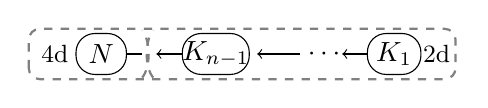
\begin{tikzpicture}[scale=1.0,baseline=(current bounding box.center)]
      % 唯一的虚线圆角框
      \draw[gray,dashed,thick,rounded corners=4pt] (0,0) rectangle (5.42,0.64);
      % 左端 4d 结点
      \node[font=\small] at (0.33,0.32) {4d};
      \draw[rounded corners=0.24cm] (0.60,0.06) rectangle (1.24,0.58);
      \node at (0.92,0.32) {$N$};
      \draw (1.24,0.32) -- (1.44,0.32);
      % 4d/2d 界面（两条对合的小弧）
      \draw[gray,dashed,thick] (1.44,0.02) .. controls (1.55,0.15) and (1.55,0.49) .. (1.44,0.62);
      \draw[gray,dashed,thick] (1.58,0.02) .. controls (1.47,0.15) and (1.47,0.49) .. (1.58,0.62);
      % 2d 链：左向箭头 + 结点
      \draw[->] (1.95,0.32) -- (1.62,0.32);
      \draw[rounded corners=0.24cm] (1.95,0.06) rectangle (2.80,0.58);
      \node at (2.375,0.32) {$K_{n-1}$};
      \draw[->] (3.45,0.32) -- (2.90,0.32);
      \node at (3.75,0.32) {$\cdots$};
      \draw[->] (4.30,0.32) -- (3.98,0.32);
      \draw[rounded corners=0.24cm] (4.30,0.06) rectangle (4.98,0.58);
      \node at (4.64,0.32) {$K_1$};
      \node[font=\small] at (5.18,0.32) {2d};
    \end{tikzpicture}
    \,\right]
    =\left\langle\hat V_{\mu_1}\hat V_{\mu_2}\hat V_{\mu_3}\hat V_{\mu_4}\right\rangle^{\text{generalization of Toda CFT}}_{S^2}
    \tag{8.10}
\end{equation}
其中 $K_i=N_1+\cdots+N_i$。虽然对称代数已被理解，但相应的、推广 Toda CFT 的（非手征）CFT 却还没有。
% [Tutor Note: p.89 (8.10) 同样是编号示意图，按 §6bis 用 TikZ 重画。读图约定与 (8.8) 相同：左边圆角矩形结点是 4d 的 $SU(N)$（纯 SYM），右边一串结点是 2d 规范群 $U(K_{n-1}),\ldots,U(K_1)$，所有箭头指向左侧，表示 2d 链逐级"收缩"进 4d 结点；界面用一对对合的灰色虚线弧表示。核对 $K_i=N_1+\cdots+N_i$：$K_n=N$，故整条 2d 链的秩正好用完 4d 规范群的秩，这正是"对称代数已被理解"的含义。]

有趣的是，仿射 $SL(2)$ 代数的共形块与带有额外退化顶点算子的 Virasoro 代数的共形块有关，这一点在 AGT 背景下很早就被指出 [600]。这一点及其 $N>2$ 的类比，导致两类面算子之间在相差一个适当积分核的意义下的某些等同 [532,601]。

阅读 2010 年代初关于 AGT 背景下表面算子的一些文献时应当小心，因为在 $\fsu(2)$ 情形下两类表面算子难以区分。这里考虑的"余维 2"轨形 $\C\times(\C/\Z_M)$ 也不应与第 83 页讨论的"余维 4"轨形 $\C^2/\Z_M$ 混淆------在后者的情形里 $\Z_M$ 转动两个因子。正如 $\C^2/\Z_M$ 轨形那样，$\C\times(\C/\Z_M)$ 轨形也应当作为 5d 规范理论在 $\C^2\times_q S^1$ 上的一个极限出现，其中 $q,t$ 取适当的单位根极限。

\subsection{畴壁}

AGT 对应也允许把 4d 时空分成两部分、或给它一个边界的半 BPS 3d 算子。一个好的出发点是 [43]。

\para{对称性破缺的壁。} 第一个构造 [43] 是把 $\cX(\fg)$ 的一个（驯服的）余维 2 缺陷放在 $S^4_b$ 的赤道上，再乘上 $C$ 中一条闭圈 $\gamma$。这个构造在规范理论中的描述，用第 84 页定义的规范群 $G_\gamma$ 来理解。4d 矢量多重态的边界条件与 GW 面缺陷附近的情形类似，它们定义了一个对称性破缺的壁：规范对称性约化为子群 $H\subset G_\gamma$。在 CFT 一侧，情形与圈算子类似，并且
